\subsection{Batterie-Antrieb}
%"In der Luftfahrt ist es möglich, direkten Strom zu nutzen. Die direkte Nutzung von
%Elektrizität erfordert Elektromotoren und Stromspeicher an Bord" \cite{dahal2021techno}, wie Batterie oder Brennstoffzellen \cite{dalmia2022powering}.
Eine andere Möglichkeit, Emissionen zu reduzieren, ist direkten Strom als Antrieb mittels Elektromotoren und Stromspeicher, wie Batterien oder Brennstoffzellen, zu nutzen.
Eine einfache Darstellung des Batterie-Antriebs (BA) ist in der Abbildung \ref{ba} gezeigt.
\begin{figure}[h]
	\centering
	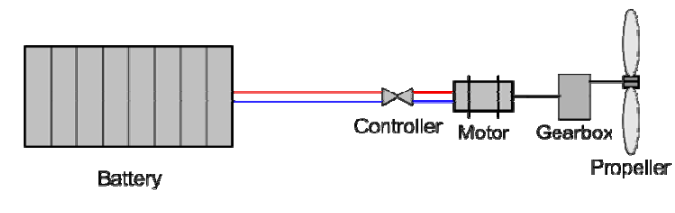
\includegraphics[width=0.7\linewidth]{Bilder/BA.png}
	\caption[Einfachster Batterie-Antrieb]{ \cite{hepperle2012electric}}
	\label{ba}
\end{figure}

Es gibt drei unterschiedliche Antriebskonfigurationen von elektrischen Flugzeugen: vollelektrisch, funktioniert nur auf der Batterie oder
Brennstoffzelle als Energiequelle, turboelektrisch und hybrid-elektrisch ist eine Mischung von konventionellen 
Gasturbinentriebwerken mit Kerosin und Batterie oder Brennstoffzellen \cite{dahal2021techno}. %Turboelelektrisches Antrieb 
Im Folgenden wird ein vollelektrischer Antrieb beschrieben.
%
Funktionsweise Elektromotor: Durch Potenzialdifferenz und einem Stromfluss wird die elektrische Energie in mechanische umgewandelt.
Im Vergleich zum Verbrennungsmotor ist der einzige bewegliche Teil bei BA der Rotor \cite{donckers2024electric}, 
was die Wartungskosten verringern kann. Außerdem besteht der elektrische Antrieb aus einem Controller, welcher den Energiefluss steuert. 
Durch den Controller wird festgelegt, welche Leistung der Motor erzeugen bzw. wie viel Energie von 
einer Batterie genutzt werden soll, um die gewünschte Leistung zu erzeugen \cite{donckers2024electric}. 

Das Batteriemanagementsystem in einem Flugzeug verfügt über Informationen wie State of Health (SOH), welche den Unterschied zwischen Anfangs-
und Bestandskapazität einer Batterie angibt, und State of Charge (SoC), welche zeigt, wie viel Prozent der verfügbaren Kapazität geladen werden kann \cite{donckers2024electric}.

%Ein Vorteil des elektrischen Flugzeugs ist, dass den Antrieb zulässt, rückwärtszufahren (Quelle) und somit auf den Schlepper-Einsatz verzichtet werden kann.
Durch die Umwandlung der elektrischen in chemische Energie kann diese in der Batterie gespeichert werden.
Im Laufe des Fluges verändern die Batterien ihr Gewicht nicht, unabhängig davon, ob sie leer oder vollständig geladen sind \cite{donckers2024electric}. 
Eine in der wissenschaftlichen Literatur weit verbreitete Batterie ist die Lithium-Ion-Batterie. Diese haben eine hohe Energiedichte im Vergleich zu anderen vorhandenen Batterien. %ist es so?
Heutige Li-ion Batterien haben eine Energiedichte von 100-265 Wh/kg (Quelle). Werden diese Werte mit der spezifischen Energiedichte von 12 kWh/kg von Kerosin verglichen \cite{dalmia2022powering},
ergibt sich eine Differenz von ca. 45-facher Steigerung gegenüber einer Li-Ion-Batterie. Das weist darauf hin, dass Batterien ein viel höheres Gewicht für die gleiche Energie verursachen. 
Somit steigt auch die Masse des Flugzeugs.

Batterien sind von äußerlichen Bedingungen beeinflussbar. Kalte Umgebungen können 
den Wirkungsgrad reduzieren (Quelle), warme Umgebungen können zu einem schnelleren Auslaufen der Lebensdauer führen.
Die Herstellung einer Lithium-Ionen-Batterie ist durch Lithium-Produktion umweltschädlich (hoher Wasserverbrauch, gefährliche Leckagen) und 
kostenintensiv in der Wartung \cite{dalmia2022powering}. 

In Forschung befinden sicht weitere Arten von Batterien wie Lithium-Sulfur, Lithium-Air, sowie Solid-state Batterien, welche vielversprechend wirken (Quelle).
%
%
%Batterien werden bereits jetzt als sekundäre Leistungsquelle.(Schmidt?)

Der Batteriewechsel ist kompatibler mit der Flugplanung, benötigt aber mehrere Batterien für den Austausch, was die Logistik erschwert 
und höhere Anschaffungskosten verursacht. Batterien müssen ordnungsgemäß und sicher gelagert werden. \cite{salucci2020optimal}

Ein Batteriewechsel ist öfters vorkommende in der Literatur Ladung.

Ladeleistung ist für die Dauer der Ladung verantwortlich. Durch schnellere Ladungen wird Lebensdauer der Batterien reduziert. Was mit sich bringt, dass die Batterien schneller ausgetauscht werden müssen
und mehr Kosten dadurch entsteht. (Quelle) Wobei die langsamen Laden ist für die Fluggesellschaften nicht rentabel sein kann, 
da wenn Flugzeug auf dem Boden steht verdienen Fluggesellschaften kein Geld.

Transportkapazität ist nicht so groß, wie bei konventionellen Flugzeugen und auch die Reichweite für Regionalflüge \cite{abrantes2024impact}.
Die Energieproduktion ist nicht emissionsfrei \cite{abrantes2024impact}, dafür muss mehr erneuerbaren Quellen hergestellt werden, 
wie Solar- und Windenergie. 
%Wasserstoff braucht kryogene Lagerung, hat Entflammbarkeit und braucht Infrastrukturentwicklung.\cite{abrantes2024impact}

In Bezug auf Sicherheit, das größte Gefahr bei BA ist chemische Reaktion des thermischen Durchgehens, wofür stabile
Kühlungssysteme benötigt sind \cite{donckers2024electric}. Thermisches Durchgehen verursacht einen starken Anstieg der 
Innentemperatur von Batterie, was zu kompletten Ausfall der Batterie oder Freisetzung der brennbaren Gase führen kann \cite{shahid2022review}.
%Das thermische Durchgehen von Lithium-Ionen-Batterien ist das Phänomen exothermer Kettenreaktionen innerhalb der Batterie.
% Diese Reaktionen verursachen normalerweise einen starken Anstieg der internen Batterietemperatur, wodurch die inneren Strukturen 
% der Batterie destabilisiert und abgebaut werden, was zu einem Totalausfall der Batterie führen kann. Das thermische Durchgehen kann 
% durch verschiedene Formen mechanischer, elektrischer und thermischer Misshandlung auftreten. All dies führt zu einem internen Kurzschluss 
% der Batterie, da der Separator zwischen Anode und Kathode entweder zusammenbricht, abreißt oder durchbohrt wird. Dadurch wird eine große 
% Menge Wärme erzeugt, die wiederum den Grad der elektrochemischen Reaktionen verstärkt und eine übermäßige Wärmeentwicklung verursacht. 
% Dieser Zyklus setzt sich fort, wodurch die Temperatur der Batterie stark ansteigt und große Mengen brennbarer Gase freigesetzt werden.
